\documentclass[journal]{IEEEtran}
\usepackage{graphicx}
\usepackage{subfigure}
\usepackage{url}
\usepackage{mathtools}
\DeclarePairedDelimiter\ceil{\lceil}{\rceil}
\DeclarePairedDelimiter\floor{\lfloor}{\rfloor}

\ifCLASSINFOpdf
\else
   \usepackage[dvips]{graphicx}
\fi
\usepackage{url}

\hyphenation{op-tical net-works semi-conduc-tor}

\usepackage{graphicx}


\begin{document}

\title{Identification of black hole states  using matrix based methods: Time series analysis of RXTE satellite data}

\author{First A. Author, \IEEEmembership{Fellow, IEEE}, Second B. Author, and Third C. Author, Jr., \IEEEmembership{Member, IEEE}
\thanks{This paragraph of the first footnote will contain the date on which you submitted your paper for review. It will also contain support information, including sponsor and financial support acknowledgment. For example, ``This work was supported in part by the U.S. Department of Commerce under Grant BS123456.'' }
\thanks{The next few paragraphs should contain the authors' current affiliations, including current address and e-mail. For example, F. A. Author is with the National Institute of Standards and Technology, Boulder, CO 80305 USA (e-mail: author@boulder.nist.gov).}
\thanks{S. B. Author, Jr., was with Rice University, Houston, TX 77005 USA. He is now with the Department of Physics, Colorado State University, Fort Collins, CO 80523 USA (e-mail: author@lamar.colostate.edu).}}

\markboth{Journal of \LaTeX\ Class Files, Vol. 14, No. 8, August 2015}
{Shell \MakeLowercase{\textit{et al.}}: Bare Demo of IEEEtran.cls for IEEE Journals}
\maketitle

\begin{abstract}
Black hole is one of the fascinating,  however mysterious, astrophysical  objects. In order to identify it one has to look at its environment, often forming a disc-like structure. This disc, called accretion disc, evolves with time transiting from one state to another. For example, in one extreme regime it shows temperature dependent radiations making the disc geometrically thin, and in yet another extreme  regime of time span however radiation turns out to be temperature independent making the disc hot and geometrically thick.  Nevertheless, in general, accretion disc lies in  states intermediate between the two extremes. The present mission is to capture black hole states  explicitly using SVD and PCA based decompositions. In order to do that we rely on time series data of black hole \textit{GRS 1915 + 105} obtained from RXTE satellite. As a black hole cannot be seen directly, identifying its states accurately could help in characterizing its properties. Earlier time series  analysis based on Correlation Integral (CI) approaches, supplemented by theory, argued for four specific states. However there are caveats when data themselves are not free from noise and the  appropriate method for such an analysis itself is exploratory. Present interdisciplinary study aims at, on one hand,  to cross-verify the previous inference, on the other hand to identify, if any,  novel characteristics of black holes. In the experiments conducted it is found that among the proposed matrix based methods, SVD analysis concurs with CI based analysis on all the 12 classes of time series utilized. However, the inference using PCA based approach illustrates that one  class among the 12 turns out to be inconsistent with the other approaches. Investigation into these (in)consistencies  is expected to have long standing implications in astrophysics and otherwise.
\end{abstract}

\begin{IEEEkeywords}
Enter key words or phrases in alphabetical order, separated by commas. For a list of suggested keywords, send a blank e-mail to keywords@ieee.org or visit \url{http://www.ieee.org/organizations/pubs/ani_prod/keywrd98.txt}
\end{IEEEkeywords}


\IEEEpeerreviewmaketitle



\section{Introduction}
One of the challenging problems in astrophysics is the understanding of black holes. As a black hole cannot be seen directly, to identify it, one has to look for its environment forming a disc-like structure by the infalling matter called accretion disc. In this work, we focus on the black hole source \textit{GRS 1915+105}, which presents several intriguing facets. It has been classified into 12 different temporal classes: $\alpha$, $\beta$, $\gamma$, $\delta$, $\lambda$, $\kappa$, $\mu$, $\nu$, $\rho$, $\phi$, $\chi$ and $\theta$ \cite{Belloni2000}, with their respective distinct time series. One of the fundamental aspects of the understanding is to determine if the black hole source is a stochastic system or a non-stochastic one. The latter one is related to the well-known turbulent nature of the system. There are several studies that utilize the Correlation Integral (CI) approach to determine the characterization of the black hole data \cite{Mukhopadhyay2004, misra2006}. However, there can also be other approaches to understanding the same data by applying, for e.g.,  matrix-based methods such as Principal Component Analysis (PCA) and Singular Value Decomposition (SVD). It is useful to compare the inferences obtained using these two distinct approaches; the implications of the (dis)similarities in inferences, if any, could lead to questions about understanding the temporal dynamics of the system.

Interestingly, to quantify the properties of a black hole source, along with temporal features one has to look for spectral features as well, they together lead to the true nature of the source. If the source radiation is temperature dependent, it produces more like a blackbody radiation, namely multicolour blackbody or ``diskbb" \cite{Shakura1973}. On the other hand, the temperature independent radiation consists of a power-law tail, named as ``PL" \cite{chakrabarti1995,narayan1994}. While the former leads the underlying accretion disc around the black hole to be geometrically thin, the latter leads to a geometrically thick disc.

In the present study, black hole states are determined by  classifying the given time series, which is photon count rate as a function of time,  as being either stochastic or non-stochastic. This classification is performed using classical matrix based methods, SVD and PCA.
However, the novelty of the study lies in (i) quantifying temporal complexity obtained by SVD decomposition, using topological techniques and (ii) utilizing features derived from PCA for classification. Based on our analysis there are four possible black hole states \cite{Adegoke2018}:
\begin{enumerate}
\item Non-stochastic and diskbb: Keplerian disc \cite{Shakura1973}.
\item Non-stochastic and PL: Advection Dominated Accretion Flow (ADAF)  \cite{narayan1994}.
\item Stochastic and diskbb: Slim disc \cite{Abramowicz1988}.
\item Stochastic and PL: General Advective Accretion Flow (GAAF) \cite{chakrabarti1995, rajesh2010}.
\end{enumerate}

Utility of the proposed approach is illustrated by comparing the results with previously established methods. Following are the major contributions of this paper:
\begin{itemize}
\item SVD decomposition of the data matrix is used for identifying the temporal dynamics of the time series as in \cite{misra2006}. A plot involving the top two right singular vectors of the data matrix shows a clear distinction between stochastic and non-stochastic time series. This distinction is captured using the topological descriptor called Betti numbers \cite{jmlr}. This descriptor for a stochastic time series is topologically simpler than that for a non-stochastic one.

\item PCA, which is a widely used approach for decorrelating features and dimensionality reduction, is utilized for characterizing a time series as stochastic vs non-stochastic. We propose a novel approach by iteratively computing eigenvalue ratios  of covariance matrix for different subintervals of the time series. We  derive multiple features from the eigenvalue ratios and use them to characterize the time series.
\end{itemize}


\section{Related Work}
Several groups have worked on distinguishing between stochastic and non-stochastic time series. The idea of utilizing Permutation Entropy (PE) to determine the complexity measure of a time series was explored in \cite{Bandt2002}. In the work reported in \cite{Boaretto2021}, PE was used to parameterize a given time series  followed by classification using  Neural Network. The paper explored the idea of utilizing PE of a time series to determine if it is strongly correlated with known stochastic signals (noise).   The claim was that for non-stochastic signals the deviation of the parameter is relatively large as compared to that of the parameter of a stochastic signal. Another set of reported studies are based on  graph theory. In the work reported in \cite{lacasa2010}, the authors have utilized the horizontal visibility algorithm in order to distinguish between stochastic and non-stochastic processes. A recent work, reported in \cite{Silva2022}, mapped time series into  graphs and computed various topological properties, which they called \textit{NetF}, capturing  measures such as centrality, distance, connectivity etc. PCA was applied on the \textit{NetF} feature matrix and clustering was performed on the principal components.

 In the approach outlined in \cite{Brunton2016}, the authors combined the idea of sparsity and machine learning with non-linear dynamical systems, in order to determine the governing dynamics. Sparse regression was used to determine the fewest terms in the equations that govern the dynamics of the phenomenon. The user-defined dictionary of basis functions consists of well-known functions such as polynomials, trigonometric functions and exponentials. However, the optimal choice of dictionary for a specific choice of problem remains a challenge.

In this work, we propose to utilize classical matrix based methods which do not require any assumptions about the underlying phenomenon.

\section{Proposed Method and Data used}

In this work, we use two different matrix based approaches, one using SVD followed by  Betti number descriptors, and  another using PCA in order to characterize time series as stochastic vs non-stochastic.

\subsection{SVD based approach}
In this approach, we form uncorrelated observation vectors from the raw time series data by utilizing the optimal value of embedding dimension \cite{misra2006}. A data matrix, $D$, is formed with each row  as the  time shifted version of the original time series. The time shift is chosen to be large enough so that each column can be viewed as a different observation vector of the same time evolving phenomenon. Temporal dynamics is understood by utilizing the right singular vectors of the SVD decomposition of $D$ as given in equation (\ref{eqn:svd}) below. Columns of $U$ and $V$  form the left and right singular vectors respectively and $\Sigma$ is a block diagonal matrix with diagonal elements as the singular values, given by
\begin{equation}
D = U \Sigma V^T.
\label{eqn:svd}
\end{equation}
We observe the plot of the top two right singular vectors (E1 vs E2). For non-stochastic time series this plot is expected to show a specific pattern (attractor behavior, where the plot follows a trajectory leaving a well-defined gap). On the other hand, for stochastic time series, this behavior is absent.

The characteristics of the E1 vs E2 plot are captured using Betti numbers \cite{jmlr}. Betti number descriptor for a $d$-dimensional manifold is a vector of $d$ integers which is represented as $\beta = (\beta_0, \beta_1 \mathellipsis \beta_{d-1})$. Here the E1 vs E2 plots are 2-d manifolds, which are described by  $\beta=(\beta_{0}, \beta_{1}$).  $\beta_{0}$ is the number of blobs (connected components) while $\beta_1$ is the number of $1$-d holes. For a stochastic time series the values of $\beta_{0}$  and $\beta_1$ are expected to be 1 and 0 respectively, as the E1 vs E2 plot consists of one single blob. However, for a non-stochastic time series, we observed that the value of $\beta_{0}$ can be greater than 1 and the value of $\beta_1$ is always greater than 0 due to the attractor behavior.


\subsection{PCA Based approach}
We utilize PCA to understand if the available data possess a dominant orientation. This can be computed by splitting the time series into two halves, and computing the covariance matrix of these observations. The eigenvalues of this $2 \times 2$ covariance matrix will show one of the signatures: If the data indeed show any dominant direction (as in non-stochastic time series), then the larger eigenvalue will be significantly greater than the other. This will lead to a large ratio of the eigenvalues. On the other hand, if the data do not show any dominant direction (as in stochastic time series), then the two eigenvalues of the covariance matrix will be comparable. This will lead to small values of eigenvalue ratio.

Consider a time series consisting of $n$ values  $z_1, z_2 \mathellipsis z_n$. We begin by computing the eigenvalue ratio for the entire series using the following steps:
\begin{itemize}
\item  Split the series into two halves $(z_1, z_2 \mathellipsis z_{\floor*{\frac{n}{2}}})$ and $(z_{\floor*{\frac{n}{2}} + 1}, \mathellipsis z_n)$.
\item Compute covariance matrix, $C$,  by treating the samples in two halves as $\floor*{\frac{n}{2}}$ observations of two dimensional vectors.
\item Find eigenvalues of $C$, $\lambda_1$ and $\lambda_2$; the eigenvalue ratio is computed as  $\lambda_1/\lambda_2$ where $\lambda_1 \ > \lambda_2$ (eigenvalues of a covariance matrix are real).
\end{itemize}
If the eigenvalue ratio for an interval is less than a predefined threshold (empirically determined as 10 for the given dataset), the interval is split into two sub-intervals of equal size and the eigenvalue ratio for each sub-interval is computed. The process is repeated as long as the length of the sub-interval is greater than a predefined number of samples.

Using PCA analysis we have derived the following three features for each time series:
\begin{itemize}
\item Maximum eigenvalue ratio (MER): This is the maximum value obtained as the ratio of the two eigenvalues of the covariance matrix of any sub-interval of the time series.
\item Variance of eigenvalue ratio (VAR): This is the variance of the eigenvalue ratios of covariance matrices across sub-interval in the entire time series.
\item Area under the eigenvalue ratio curve (Area): This measure captures the area under the curve of the eigenvalue ratio for the entire time series.
\end{itemize}

\subsection{Data used}
The proposed approaches are illustrated on the publicly available data of \textit{GRS 1915 + 105} taken from website \cite{xte}. 12 distinct classes of time series are utilized from the available data. All these time series are re-sampled with a sampling interval of 0.1 second. These datasets  were  also used in the work reported in \cite{Adegoke2018}, where the authors use CI based approaches, leading us to be able to compare our obtained results with theirs. Figures \ref{phi_ts} and \ref{theta_ts} show a representative time series of stochastic and non-stochastic  nature respectively.

%\begin{figure}[ht]
%\centering
%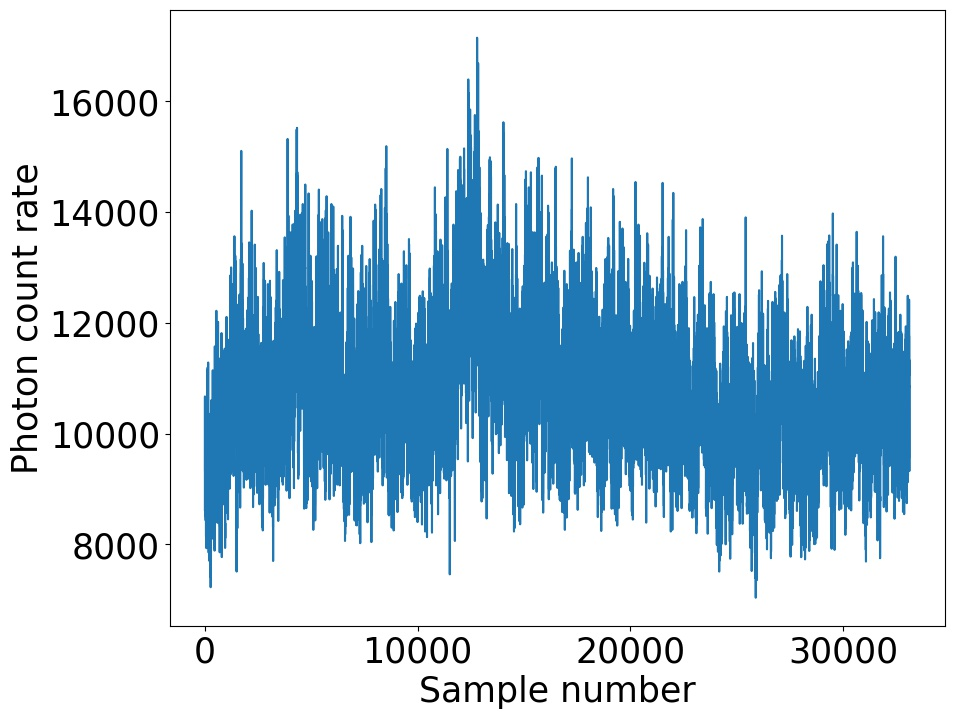
\includegraphics[width=0.8\linewidth]{sac_ascf_phi.jpg}
%\caption{A representative stochastic time series of class $\phi$ of \textit{GRS 1915 + 105}. X-axis: Sample number (Scale: 0 - 35000), Y-axis: Photon count rate (Scale: 0 - 18000). }
%\label{phi_ts}
%\end{figure}
%
%\begin{figure}[ht]
%\centering
%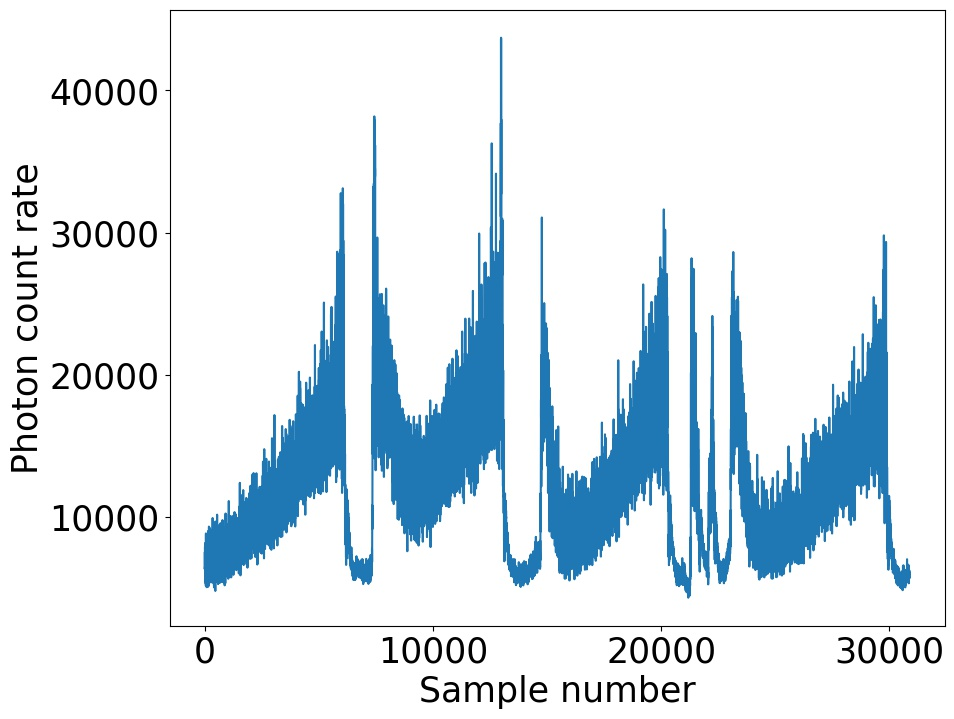
\includegraphics[width=0.8\linewidth]{sac_ascf_theta.jpg}
%\caption{A representative non-stochastic time series of class $\theta$ of \textit{GRS 1915 + 105}. X-axis: Sample number (Scale: 0 - 35000), Y-axis: Photon count rate (Scale: 0 - 45000). }
%\label{theta_ts}
%\end{figure}

\section{Results and Discussion}

\subsection{Results of SVD based analysis}


%From SVD decomposition of the data matrix, we pick up the top 2 right singular vectors (E1, E2) corresponding to the temporal dynamics and plot E1 vs E2 for each time series. Figure \ref{svd_e1e2_nonstochastic} shows the panel of representative E1-E2 plots for time series  that are classified as non-stochastic and Figure \ref{svd_e1e2_stochastic}  shows the corresponding panels for time series that are classified as stochastic. The Betti number descriptors for each of the E1-E2 plots are tabulated in Table \ref{tab:results} under the column Betti descriptors. In order to infer the label of the time series from the Betti descriptors, We use the following strategy. Betti descriptor $\beta = (\beta_0, \beta_1)$. We use the L1-norm of $\beta$. If $\lvert \beta \rvert \gt 1$ then the time series is classified as non-stochastic else the time series is stochastic.

From SVD decomposition of the data matrix, we plot the top 2 right singular vectors (E1 vs E2) to understand the temporal dynamics for each time series. Figure \ref{svd_e1e2_nonstochastic} shows representative E1 vs E2 plots for time series  that are classified as non-stochastic and Figure \ref{svd_e1e2_stochastic}  shows the corresponding plots for time series that are classified as stochastic. The Betti number descriptors for each of the E1 vs E2 plots are tabulated in Table \ref{tab:results} under the column \textit{Betti descriptor}. In order to infer the label of the time series from the Betti descriptors, we use the L1-norm of $\beta$, $\|\beta\|_1$. If $\|\beta\|_1 > 1$, the time series is classified as non-stochastic, else the time series is stochastic.


%\begin{figure*}
%  \centering
%  \subfigure[]{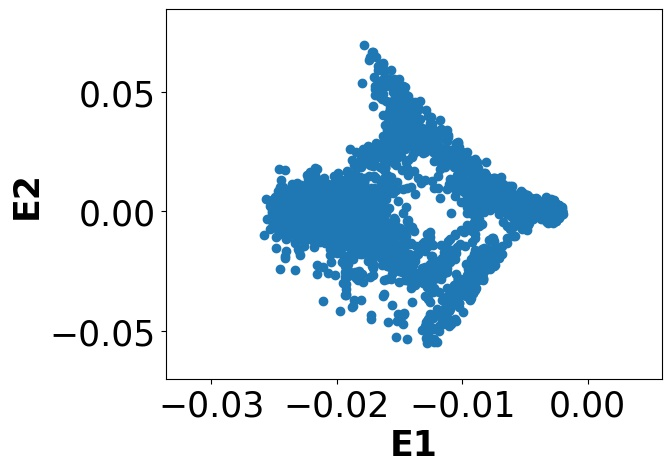
\includegraphics[width=0.25\textwidth]{images/sac_ascf_kappa_e1_vs_e2_m_2_tau_50.jpg}}
%  \subfigure[]{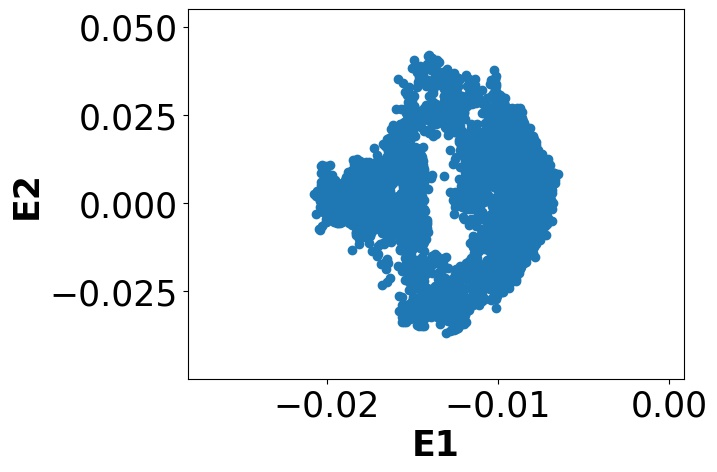
\includegraphics[width=0.25\textwidth]{images/sac_ascf_mu_e1_vs_e2_m_4_tau_80.jpg}}
%  \subfigure[]{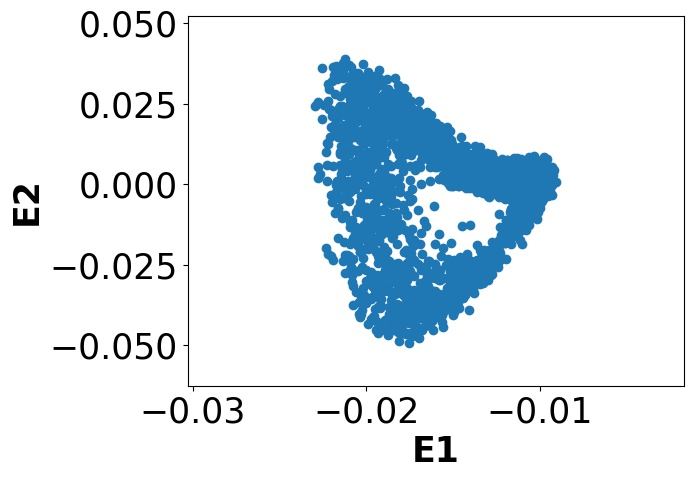
\includegraphics[width=0.25\textwidth]{images/sac_ascf_rho_e1_vs_e2_m_8_tau_20.jpg}}
%  \caption{Plot of E1 vs E2 (top two right singular vectors) of data matrix for  representatives from non-stochastic time series of \textit{GRS 1915 + 105}. The series are $\kappa$, $\mu$ and $\rho$ from left to right.}
%  \label{svd_e1e2_nonstochastic}
%\end{figure*}



%\begin{figure*}
%  \centering
%  \subfigure[]{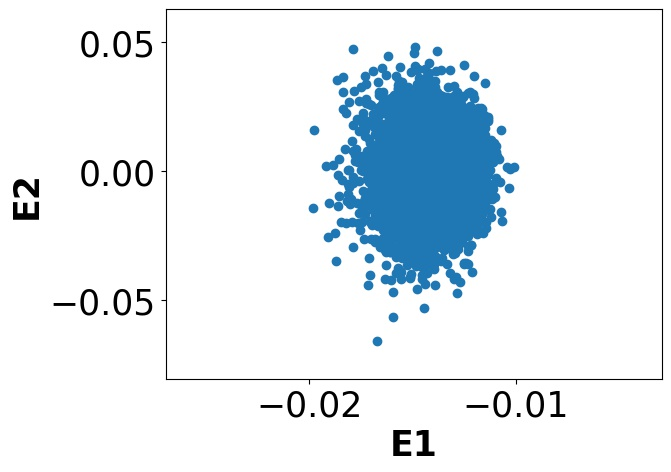
\includegraphics[width=0.25\textwidth]{images/sac_ascf_phi_e1_vs_e2_m_2_tau_20.jpg}}
%  \subfigure[]{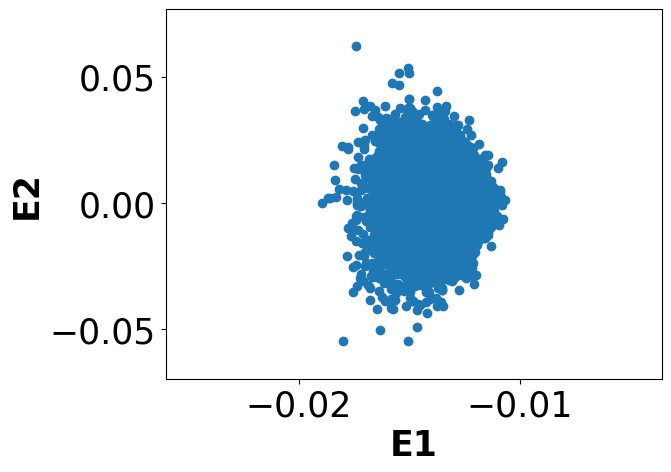
\includegraphics[width=0.25\textwidth]{images/sac_ascf_kai_e1_vs_e2_m_2_tau_20.jpg}}
%  \subfigure[]{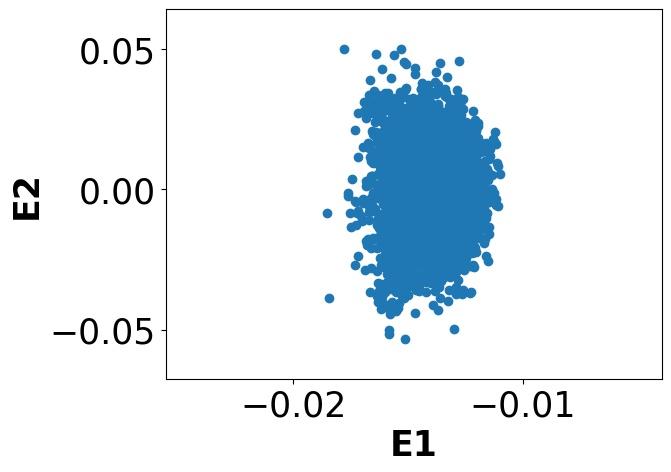
\includegraphics[width=0.25\textwidth]{images/sac_ascf_gamma_e1_vs_e2_m_2_tau_20.jpg}}
%\caption{Plot of E1 vs E2 (top two right singular vectors) of data matrix for  representatives from  stochastic time series  of \textit{GRS 1915 + 105}. The series are $\phi$, $\chi$ and $\gamma$ from left to right.}
%  \label{svd_e1e2_stochastic}
%\end{figure*}


\subsection{Results of PCA based analysis}

%\begin{figure}[ht]
%\centering
%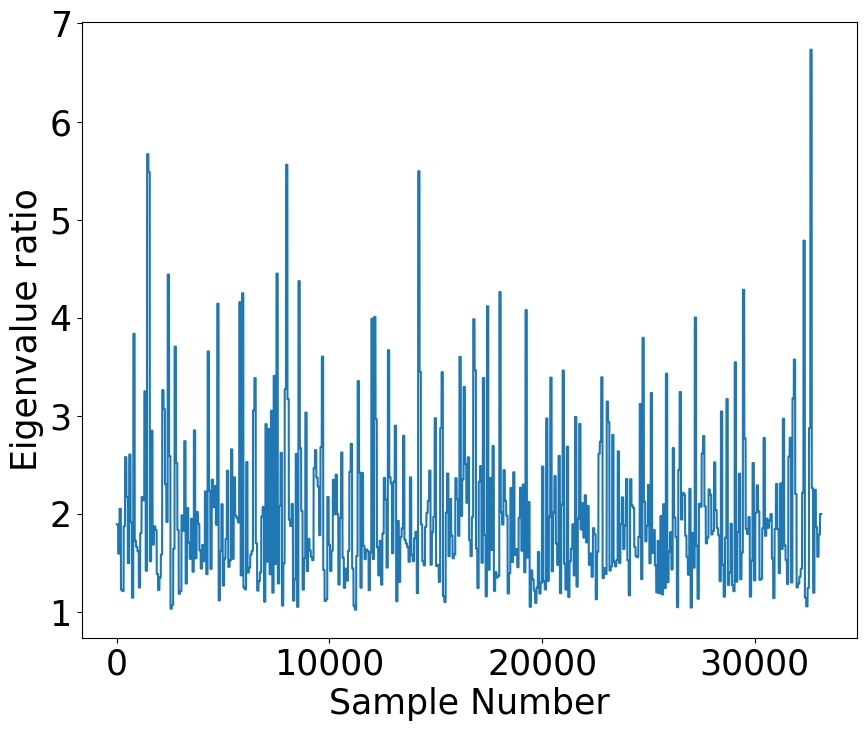
\includegraphics[width=0.8\linewidth]{sac_ascf_phi_eig.jpg}
%\caption{Plot of eigenvalue ratio of the stochastic time series shown in Figure \ref{phi_ts}. X-axis: Sample number (Scale: 0 - 35000), Y-axis: Eigenvalue ratio (scale- 0 - 7). MER=7}
%\label{phi_eig}
%\end{figure}
%
%\begin{figure}[ht]
%\centering
%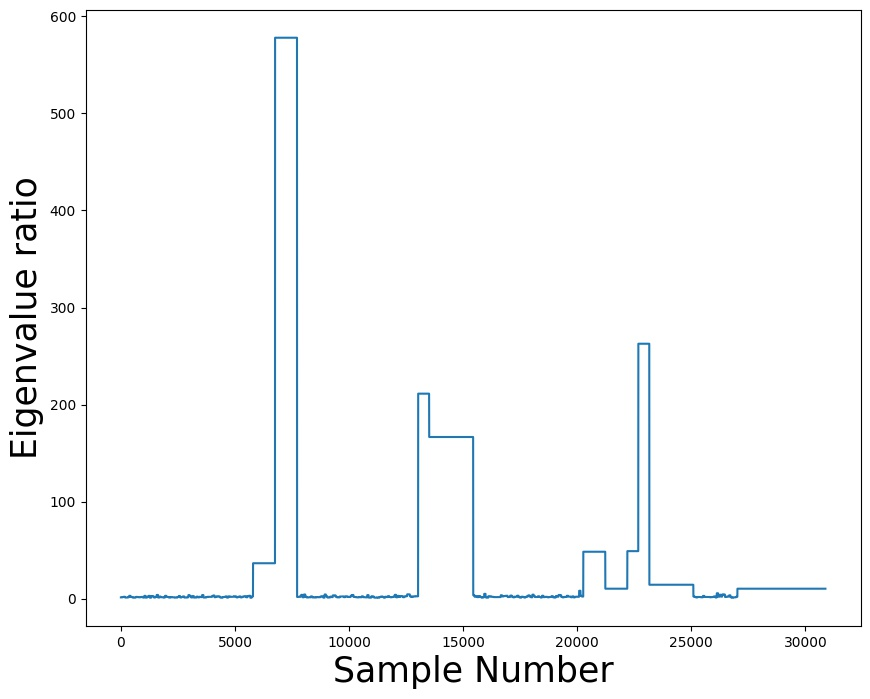
\includegraphics[width=0.8\linewidth]{sac_ascf_theta_eig.jpg}
%\caption{Plot of eigenvalue ratio of the  non-stochastic time series shown in Figure \ref{theta_ts}. X-axis: Sample number (Scale: 0 - 35000), Y-axis: Eigenvalue ratio (scale- 0 - 600). MER=577 }
%\label{theta_eig}
%\end{figure}

Figures \ref{phi_eig} and \ref{theta_eig} show the eigenvalue ratio plots for stochastic time series shown in Figure \ref{phi_ts} and  non-stochastic time series shown in Figure \ref{theta_ts} respectively. We compute the three PCA based features which are MER, VAR and Area  and utilize them for classification using the following observations:

\begin{itemize}
\item MER: For stochastic time series, eigenvalue ratios  are small across the entire time series, typically lying in the range 1-20. This implies that MER  will also be small. On the other hand, for  non-stochastic time series the eigenvalue ratios are significantly high, typically reaching a few hundreds in certain sub-intervals. Hence the MER for a non-stochastic time series is typically large.
\item VAR: For a stochastic signal since the range of eigenvalue ratios is typically small, the VAR is also small. On the other hand, for a non-stochastic signal, since the eigenvalue ratios occupy a large range of values, VAR is typically high.
\item Area: For a stochastic time series, since the eigenvalue ratios  are small the Area is also small. However, for a non-stochastic signal the eigenvalue ratios remain high for longer time intervals. Hence the Area is significantly higher.
\end{itemize}

\subsection{Consolidated Results}

Table \ref{tab:results}  tabulates the computed features and the respective inferences using the proposed approaches. Comparison of our results with CI based approach \cite{Adegoke2018} is also presented. The columns of the table are described below.

\begin{enumerate}
\item Column 1 (\textit{Class}) gives the class of the time series \cite{Adegoke2018}.
\item Column 2 (\textit{diskbb}) and column 3 (\textit{PL}) give quantities diskbb and  PL, respectively, which indicate the spectral states of the black hole \cite{Adegoke2018}.
\item Column 4 (CI Inference) gives the inference about the state of the time series using CI approach \cite{Adegoke2018}.
\item Column 5 (Betti descriptor) gives the Betti description of the E1 vs E2 plots and column 6 gives the SVD based inference.
\item The computed PCA based features: MER, VAR and Area  are tabulated in columns 7, 8 and 9 respectively. Our inference using these PCA features is given in column 10.
\item Finally the last column gives if there is a match between all three inferences.
\end{enumerate}


\begin{table*}[t]
\caption{Timeseries: Comparison between CI based label and inference using proposed approaches. The mismatched time series class, $\delta$, is shown in bold. (LC stands for Limit Cycle \cite{Adegoke2018} which is non-stochastic, $F$ stands for Fractal which is also non-stochastic and $S$ stands for stochastic)}
\begin{center}
\begin{tabular}{|p{0.5cm}|p{0.75cm}|p{0.75cm}|p{1cm}|p{2.5cm}|p{3cm}|p{0.75cm}|p{1cm}|p{0.5cm}|p{1.8cm}|p{0.75cm}|}
\hline
Class & diskbb & PL  & CI \newline Inference & Betti descriptor & SVD  \newline Inference & MER & Variance & Area & PCA \newline Inference  &  Match \\
\hline
$\beta$ & 46 & 52 & F & (1,3) & Non-stochastic & 214 & 483 & 43 & Non-stochastic & Yes\\
\hline
$\theta$  & 11 &  88 & F & (3, 2) & Non-stochastic & 577 & 778 & 58&Non-stochastic  &  Yes \\
\hline
$\lambda$ &  54 & 46 & F & (1,3) & Non-stochastic & 600 & 6782 & 314 & Non-stochastic & Yes \\
\hline
$\kappa$ &  59 & 51 & F & (1,3) & Non-stochastic & 700 & 5199 & 144 & Non-stochastic &  Yes \\
\hline
$\mu$  & 56 & 41 & F & (1,1) & Non-stochastic & 50 & 51 & 12 & Non-stochastic & Yes \\
\hline
$\nu$  & 28 & 72 & F & (1,6) & Non-stochastic & 30 & 32 & 16 & Non-stochastic & Yes\\
\hline
$\alpha$  & 23 & 77& F & (6,0 ) & Non-stochastic & 30 & 1.9 & 27.7 & Non-stochastic & Yes \\
\hline
$\rho$  & 28 & 72 & LC & (1,1) &  Non-stochastic & 60 & 147 & 35 & Non-stochastic & Yes \\
\hline
\textbf{$\delta$}  & \textbf{48} & \textbf{50} &  \textbf{S} & \textbf{(1,0)}& \textbf{Stochastic}& \textbf{42} & \textbf{9.74} & \textbf{26.2} & \textbf{Non-stochastic} &  \textbf{No} \\
\hline
$\phi$  & 50 & 34 & S & (1,0)& Stochastic & 7 & 0.5 & 15 & Stochastic &  Yes \\
\hline
$\gamma$  & 60 & 31 & S & (1,0)& Stochastic & 12 & 1 & 16 & stochastic &  Yes \\
\hline
$\chi$  & 09 & 89 & S & (1,0)& Stochastic & 5.6 & 0.25 & 6.05 & Stochastic &  Yes \\
\hline
\end{tabular}
\label{tab:results}
\end{center}
\end{table*}

%\begin{figure}
% \centering
% 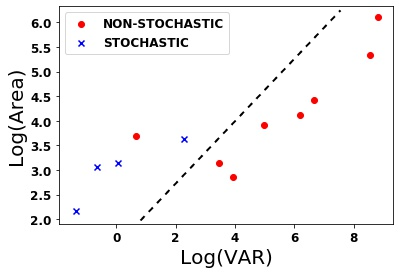
\includegraphics[width=.8\linewidth]{variance_area.drawio.png}
% \caption{Feature space (VAR and Area) shows that the two classes are well separated. The dashed line shows the decision boundary separating the two classes. The label of one of the time series is ambiguous.}
% \label{fig:variance_area_fs}
%\end{figure}

We observe that SVD based analysis results in classification  are consistent with CI based results for all the 12 classes of time series. However, with PCA based approach the inference for  $\delta$ time series is not consistent with the other two approaches. We observe that the PCA based features, VAR and Area, result in visible clustering as shown in Figure \ref{fig:variance_area_fs}. This could be attributed to the fact that   these features take into account the entire span of time series and hence form robust feature space. According to the CI based analysis $\delta$ turns out to be in between states slim disc  and GAAF \cite{Adegoke2018}. However, the present analysis shows that $\delta$ falls in between ADAF and Keplerian disc.


\section{Conclusion}
Exploring different techniques in order to have a conclusive inference for black hole systems turns out to be indispensable. We explore two different classical matrix based techniques to identify states of \textit{GRS 1915+105} black hole using the time series obtained from \textit{RXTE} satellite data. Based on our analysis, we are able to identify two extreme temporal dynamical classes of accretion around black holes. In the first approach we extend  SVD decomposition to understand temporal dynamics,  by adding  topological descriptors, to classify time series as stochastic vs non-stochastic. In yet another approach, a novel application of  PCA  to characterize the time series is proposed. We compare inferences of the CI based approach with those obtained using the proposed matrix based methods. Of the 12 classes of time series analysed, a mismatch is observed in the PCA based inference of only one class, while all other classes concur.

\section*{Acknowledgment}

The preferred spelling of the word ``acknowledgment'' in American English is without an ``e'' after the ``g.'' Use the singular heading even if you have many acknowledgments. Avoid expressions such as ``One of us (S.B.A.) would like to thank . . . .'' Instead, write “F. A. Author thanks ... .” In most cases, sponsor and financial support acknowledgments are placed in the unnumbered footnote on the first page, not here.

\section*{References and Footnotes}

\subsection{References}

References need not be cited in text. When they are, they appear on the line, in square brackets, inside the punctuation.  Multiple references are each numbered with separate brackets. When citing a section in a book, please give the relevant page numbers. In text, refer simply to the reference number. Do not use ``Ref.'' or ``reference'' except at the beginning of a sentence: ``Reference [3] shows . . . .'' Please do not use automatic endnotes in {\em Word}, rather, type the reference list at the end of the paper using the ``References'' style.

Reference numbers are set flush left and form a column of their own, hanging out beyond the body of the reference. The reference numbers are on the line, enclosed in square brackets. In all references, the given name of the author or editor is abbreviated to the initial only and precedes the last name. Use them all; use {\em et al.} only if names are not given. Use commas around Jr., Sr., and III in names. Abbreviate conference titles.  When citing IEEE transactions, provide the issue number, page range, volume number, year, and/or month if available. When referencing a patent, provide the day and the month of issue, or application. References may not include all information; please obtain and include relevant information. Do not combine references. There must be only one reference with each number. If there is a URL included with the print reference, it can be included at the end of the reference.

Other than books, capitalize only the first word in a paper title, except for proper nouns and element symbols. For papers published in translation journals, please give the English citation first, followed by the original foreign-language citation. See the end of this document for formats and examples of common references. For a complete discussion of references and their formats, see the IEEE style manual at www.ieee.org/authortools.

\subsection{Footnotes}

Number footnotes separately in superscripts (Insert $\mid$ Footnote).\footnote{It is recommended that footnotes be avoided (except for the unnumbered footnote with the receipt date on the first page). Instead, try to integrate the footnote information into the text.}  Place the actual footnote at the bottom of the column in which it is cited; do not put footnotes in the reference list (endnotes). Use letters for table footnotes (see Table I). 


\section*{References}

\subsection*{Basic format for books:}

J. K. Author, ``Title of chapter in the book,'' in {\em Title of His Published Book}, xth ed. City of Publisher, (only U.S. State), Country: Abbrev. of Publisher, year, ch. x, sec. x, pp. xxx--xxx.

\subsection*{Examples:}
\def\refname{}
\begin{thebibliography}{34}

\bibitem{}G. O. Young, ``Synthetic structure of industrial plastics,'' in {\em Plastics}, 2nd ed., vol. 3, J. Peters, Ed. New York, NY, USA: McGraw-Hill, 1964, pp. 15--64.

\bibitem{}W.-K. Chen, {\it Linear Networks and Systems}. Belmont, CA, USA: Wadsworth, 1993, pp. 123--135.

\end{thebibliography}

\subsection*{Basic format for periodicals:}

J. K. Author, ``Name of paper,'' Abbrev. Title of Periodical, vol. x,   no. x, pp. xxx--xxx, Abbrev. Month, year, DOI. 10.1109.XXX.123--456.

\subsection*{Examples:}

\begin{thebibliography}{34}
\setcounter{enumiv}{2}

\bibitem{}J. U. Duncombe, ``Infrared navigation Part I: An assessment of feasibility,'' {\em IEEE Trans. Electron Devices}, vol. ED-11, no. 1, pp. 34--39, Jan. 1959,10.1109/TED.2016.2628402.

\bibitem{}E. P. Wigner, ``Theory of traveling-wave optical laser,''
{\em Phys. Rev.},  vol. 134, pp. A635--A646, Dec. 1965.

\bibitem{}E. H. Miller, ``A note on reflector arrays,'' {\em IEEE Trans. Antennas Propagat.}, to be published.
\end{thebibliography}


\subsection*{Basic format for reports:}

J. K. Author, ``Title of report,'' Abbrev. Name of Co., City of Co., Abbrev. State, Country, Rep. xxx, year.

\subsection*{Examples:}
\begin{thebibliography}{34}
\setcounter{enumiv}{5}

\bibitem{} E. E. Reber, R. L. Michell, and C. J. Carter, ``Oxygen absorption in the earth’s atmosphere,'' Aerospace Corp., Los Angeles, CA, USA, Tech. Rep. TR-0200 (4230-46)-3, Nov. 1988.

\bibitem{} J. H. Davis and J. R. Cogdell, ``Calibration program for the 16-foot antenna,'' Elect. Eng. Res. Lab., Univ. Texas, Austin, TX, USA, Tech. Memo. NGL-006-69-3, Nov. 15, 1987.
\end{thebibliography}

\subsection*{Basic format for handbooks:}

{\em Name of Manual/Handbook}, x ed., Abbrev. Name of Co., City of Co., Abbrev. State, Country, year, pp. xxx--xxx.

\subsection*{Examples:}

\begin{thebibliography}{34}
\setcounter{enumiv}{7}

\bibitem{} {\em Transmission Systems for Communications}, 3rd ed., Western Electric Co., Winston-Salem, NC, USA, 1985, pp. 44--60.

\bibitem{} {\em Motorola Semiconductor Data Manual}, Motorola Semiconductor Products Inc., Phoenix, AZ, USA, 1989.
\end{thebibliography}

\subsection*{Basic format for books (when available online):}

J. K. Author, ``Title of chapter in the book,'' in {\em Title of Published Book}, xth ed. City of Publisher, State, Country: Abbrev. of Publisher, year, ch. x, sec. x, pp. xxx xxx. [Online]. Available: http://www.web.com 

\subsection*{Examples:}

\begin{thebibliography}{34}
\setcounter{enumiv}{9}

\bibitem{}G. O. Young, ``Synthetic structure of industrial plastics,'' in Plastics, vol. 3, Polymers of Hexadromicon, J. Peters, Ed., 2nd ed. New York, NY, USA: McGraw-Hill, 1964, pp. 15--64. [Online]. Available: http://www.bookref.com. 

\bibitem{} {\em The Founders Constitution}, Philip B. Kurland and Ralph Lerner, eds., Chicago, IL, USA: Univ. Chicago Press, 1987. [Online]. Available: http://press-pubs.uchicago.edu/founders/

\bibitem{} The Terahertz Wave eBook. ZOmega Terahertz Corp., 2014. [Online]. Available: http://dl.z-thz.com/eBook/zomega\_ebook\_pdf\_1206\_sr.pdf. Accessed on: May 19, 2014. 

\bibitem{} Philip B. Kurland and Ralph Lerner, eds., {\em The Founders Constitution}. Chicago, IL, USA: Univ. of Chicago Press, 1987, Accessed on: Feb. 28, 2010, [Online] Available: http://press-pubs.uchicago.edu/founders/ 
\end{thebibliography}

\subsection*{Basic format for journals (when available online):}

J. K. Author, ``Name of paper,'' {\em Abbrev. Title of Periodical}, vol. x, no. x, pp. xxx--xxx, Abbrev. Month, year. Accessed on: Month, Day, year, doi: 10.1109.XXX.123456, [Online].

\subsection*{Examples:}

\begin{thebibliography}{34}
\setcounter{enumiv}{13}

\bibitem{}J. S. Turner, ``New directions in communications,'' {\em IEEE J. Sel. Areas Commun.}, vol. 13, no. 1, pp. 11--23, Jan. 1995. 

\bibitem{} W. P. Risk, G. S. Kino, and H. J. Shaw, ``Fiber-optic frequency shifter using a surface acoustic wave incident at an oblique angle,'' {\em Opt. Lett.}, vol. 11, no. 2, pp. 115--117, Feb. 1986.

\bibitem{} P. Kopyt {\em et al.}, ``Electric properties of graphene-based conductive layers from DC up to terahertz range,'' {\em IEEE THz Sci. Technol.}, to be published. doi: 10.1109/TTHZ.2016.2544142.
\end{thebibliography}

\subsection*{Basic format for papers presented at conferences (when available online):}

J.K. Author. (year, month). Title. presented at abbrev. conference title. [Type of Medium]. Available: site/path/file

\subsection*{Example:}

\begin{thebibliography}{34}
\setcounter{enumiv}{16}

\bibitem{}PROCESS Corporation, Boston, MA, USA. Intranets: Internet technologies deployed behind the firewall for corporate productivity. Presented at INET96 Annual Meeting. [Online]. Available: http://home.process.com/Intranets/wp2.htp
\end{thebibliography}

\subsection*{Basic format for reports  and  handbooks (when available online):}
  
J. K. Author. ``Title of report,'' Company. City, State, Country. Rep. no., (optional: vol./issue), Date. [Online] Available: site/path/file 

\subsection*{Examples:}

\begin{thebibliography}{34}
\setcounter{enumiv}{17}

\bibitem{}R. J. Hijmans and J. van Etten, ``Raster: Geographic analysis and modeling with raster data,'' R Package Version 2.0-12, Jan. 12, 2012. [Online]. Available: http://CRAN.R-project.org/package=raster 

\bibitem{}Teralyzer. Lytera UG, Kirchhain, Germany [Online]. Available: http://www.lytera.de/Terahertz\_THz\_Spectroscopy.php?id=home, Accessed on: Jun. 5, 2014.
\end{thebibliography}

\subsection*{Basic format for computer programs and electronic documents (when available online):}

Legislative body. Number of Congress, Session. (year, month day). {\em Number of bill or resolution, Title}. [Type of medium]. Available: site/path/file
{\em NOTE:} ISO recommends that capitalization follow the accepted practice for the language or script in which the information is given.

\subsection*{Example:}

\begin{thebibliography}{34}
\setcounter{enumiv}{19}

\bibitem{}U. S. House. 102nd Congress, 1st Session. (1991, Jan. 11). {\em H. Con. Res. 1, Sense of the Congress on Approval of Military Action}. [Online]. Available: LEXIS Library: GENFED File: BILLS 
\end{thebibliography}

\subsection*{Basic format for patents (when available online):}

Name of the invention, by inventor’s name. (year, month day). Patent Number [Type of medium]. Available:site/path/file

\subsection*{Example:}

\begin{thebibliography}{34}
\setcounter{enumiv}{20}

\bibitem{}Musical tooth brush with mirror, by L. M. R. Brooks. (1992, May 19). Patent D 326 189
[Online]. Available: NEXIS Library: LEXPAT File:   DES 

\end{thebibliography}

\subsection*{Basic format for conference proceedings (published):}

J. K. Author, ``Title of paper,'' in {\em Abbreviated Name of Conf.}, City of Conf., Abbrev. State (if given), Country, year, pp. xxx--xxx.

\subsection*{Example:}

\begin{thebibliography}{34}
\setcounter{enumiv}{21}

\bibitem{}D. B. Payne and J. R. Stern, ``Wavelength-switched passively coupled single-mode optical network,'' in {\em Proc. IOOC-ECOC}, Boston, MA, USA, 1985,
pp. 585--590.

\end{thebibliography}

\subsection*{Example for papers presented at conferences (unpublished):}

\begin{thebibliography}{34}
\setcounter{enumiv}{22}

\bibitem{}D. E behard and E. Voges, ``Digital single sideband detection for inter ferometric sensors,'' presented at the {\em 2nd Int. Conf. Optical Fiber Sensors}, Stuttgart, Germany, Jan. 2--5, 1984.
\end{thebibliography}

\subsection*{Basic formatfor patents:}

J. K. Author, ``Title of patent,'' U. S. Patent x xxx xxx, Abbrev. Month, day, year.

\subsection*{Example:}

\begin{thebibliography}{34}
\setcounter{enumiv}{23}

\bibitem{}G. Brandli and M. Dick, ``Alternating current fed power supply,'' U. S. Patent 4 084 217, Nov. 4, 1978.
\end{thebibliography}

\subsection*{Basic format for theses (M.S.) and dissertations (Ph.D.):}

a) J. K. Author, ``Title of thesis,'' M. S. thesis, Abbrev. Dept., Abbrev. Univ., City of Univ., Abbrev. State, year.

b) J. K. Author, ``Title of dissertation,'' Ph.D. dissertation, Abbrev. Dept., Abbrev. Univ., City of Univ., Abbrev. State, year.

\subsection*{Examples:}

\begin{thebibliography}{34}
\setcounter{enumiv}{24}

\bibitem{}J. O. Williams, ``Narrow-band analyzer,'' Ph.D. dissertation, Dept. Elect. Eng., Harvard Univ., Cambridge, MA, USA, 1993.

\bibitem{}N. Kawasaki, ``Parametric study of thermal and chemical nonequilibrium nozzle flow,'' M.S. thesis, Dept. Electron. Eng., Osaka Univ., Osaka, Japan, 1993.
\end{thebibliography}

\subsection*{Basic format for the most common types of unpublished references:}

a) J. K. Author, private communication, Abbrev. Month, year.

b) J. K. Author, ``Title of paper,'' unpublished.

c) J. K. Author, ``Title of paper,'' to be published.

\subsection*{Examples:}

\begin{thebibliography}{34}
\setcounter{enumiv}{26}

\bibitem{}A. Harrison, private communication, May 1995.

\bibitem{}B. Smith, ``An approach to graphs of linear forms,'' unpublished.

\bibitem{}A. Brahms, ``Representation error for real numbers in binary computer arithmetic,'' IEEE Computer Group Repository, Paper R-67-85.
\end{thebibliography}

\subsection*{Basic formats for standards:}

a) {\em Title of Standard}, Standard number, date.

b) {\em Title of Standard}, Standard number, Corporate author, location, date.

\subsection*{Examples:}

\begin{thebibliography}{34}
\setcounter{enumiv}{29}


\bibitem{}IEEE Criteria for Class IE Electric Systems, IEEE Standard 308, 1969.

\bibitem{} Letter Symbols for Quantities, ANSI Standard Y10.5-1968.
\end{thebibliography}

\subsection*{Article number in reference examples:}

\begin{thebibliography}{34}
\setcounter{enumiv}{31}

\bibitem{}R. Fardel, M. Nagel, F. Nuesch, T. Lippert, and A. Wokaun, ``Fabrication of organic light emitting diode pixels by laser-assisted forward transfer,'' {\em Appl. Phys. Lett.}, vol. 91, no. 6, Aug. 2007, Art. no. 061103. 

\bibitem{} J. Zhang and N. Tansu, ``Optical gain and laser characteristics of InGaN quantum wells on ternary InGaN substrates,'' {\em IEEE Photon.} J., vol. 5, no. 2, Apr. 2013, Art. no. 2600111
\end{thebibliography}

\subsection*{Example when using et al.:}

\begin{thebibliography}{34}
\setcounter{enumiv}{33}

\bibitem{}S. Azodolmolky {\em et al.}, Experimental demonstration of an impairment aware network planning and operation tool for transparent/translucent optical networks,'' {\em J. Lightw. Technol.}, vol. 29, no. 4, pp. 439--448, Sep. 2011.
\end{thebibliography}

\end{document}
